\section{System Description}
The system was named CELINE, an abbreviation that comes from the descriptive phrase ``\textbf{C}ode \textbf{E}va\textbf{L}uation \textbf{I}n .\textbf{NE}t'' (the uppercase bolded letters forming the abbreviation). Figure \ref{fig:SystemOverview} describes an overview of the system. The system uses a web based GUI for listing problems and submitting solutions to them.

\begin{figure}[h]
	\centering
	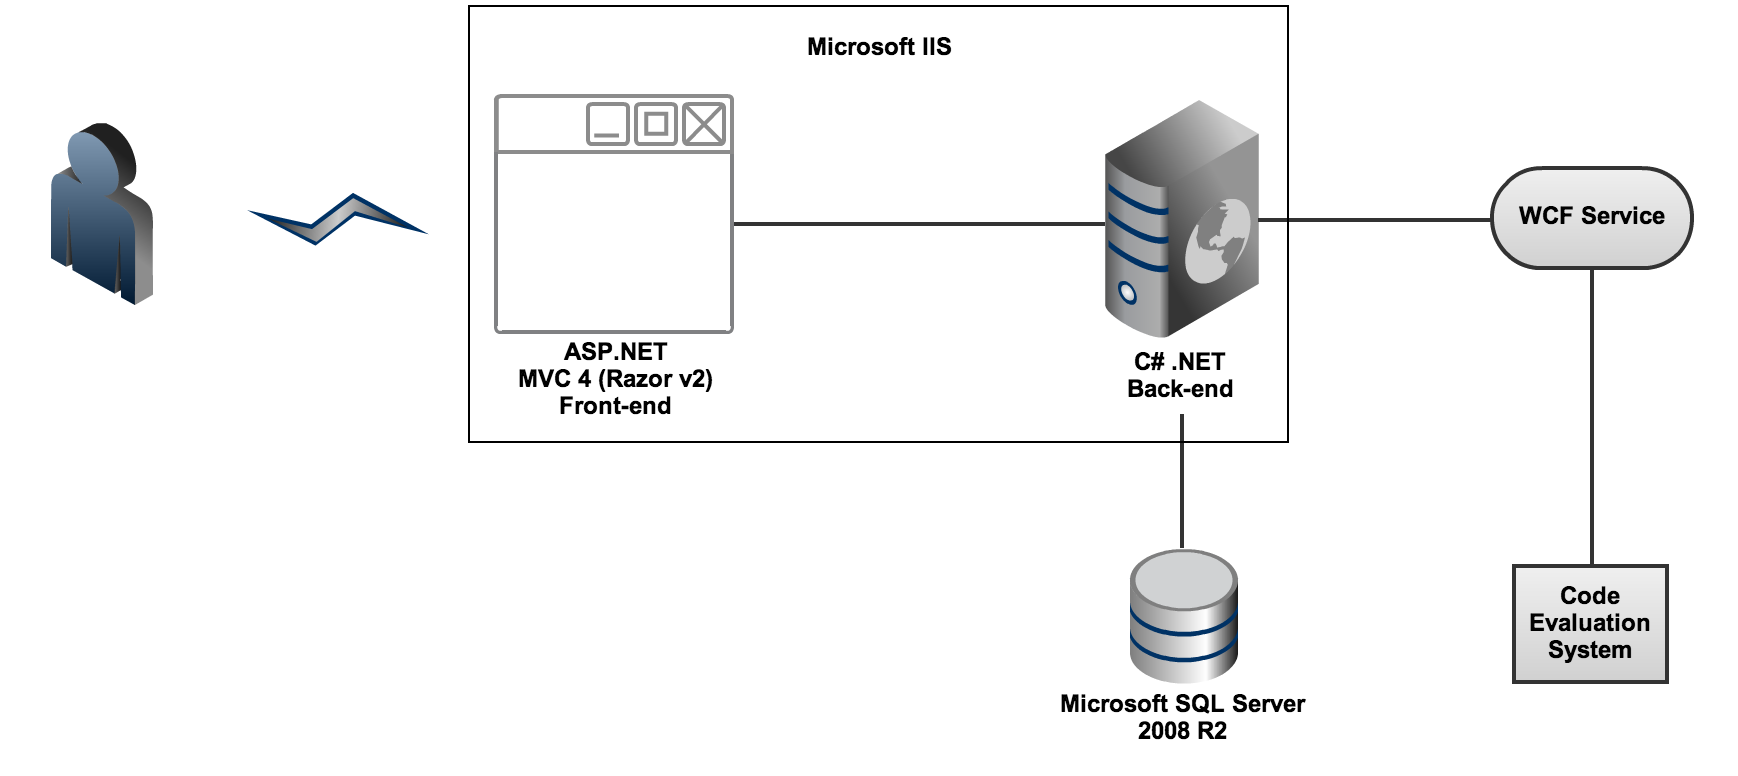
\includegraphics[width=\linewidth]{chapters/media/overview.png}
	\caption{Overview of CELINE.}
	\label{fig:SystemOverview}
\end{figure}

Going through this figure from left to right we can see that a user connects to the website through a web based GUI, which is built using a combination of ASP.NET MVC4 (Razor v2) technology and JavaScript. The system uses Microsoft IIS to enable this web support, which the standard web server software used in .NET. When the user submits code to solve a problem, that submission is saved to a database which is a Microsoft SQL Server 2008 R2 database. The submission is then forwarded to a WCF Service which in turn creates a new instance of the code evaluation system (built using C\#) using the submission as input. It then returns the status code generated from the submission, this is described in section \ref{subsec:status_codes}.


\subsection{The Web GUI}
The GUI is built using the ASP.NET MVC4 template. This saved both time and effort while still giving the website an easy to understand simplistic style. 

\begin{figure}[h]
	\centering
	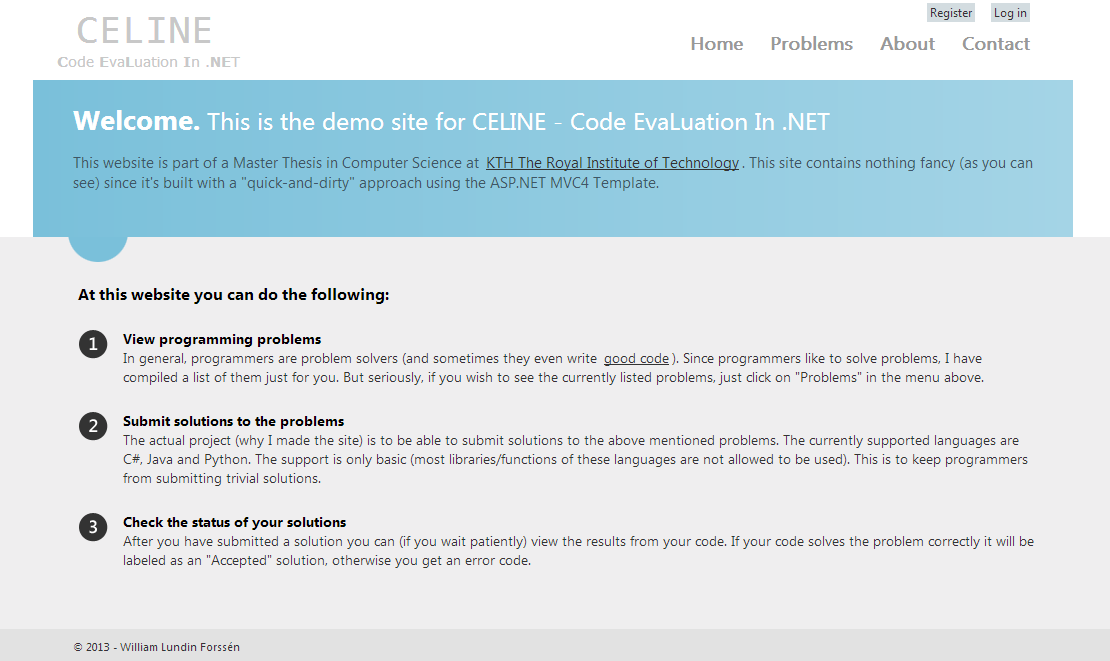
\includegraphics[width=0.75\textwidth]{chapters/media/celine_startpage.png}
	\caption{The start page of CELINE.}
	\label{fig:celine_startpage}
\end{figure}

In Figure \ref{fig:celine_startpage} we see the start page. The middle area contains some informative text, the top right contains the site menu, the register and login buttons.

\begin{figure}[h]
\centering
\mbox{
	\subfigure[List of available problems.]{
		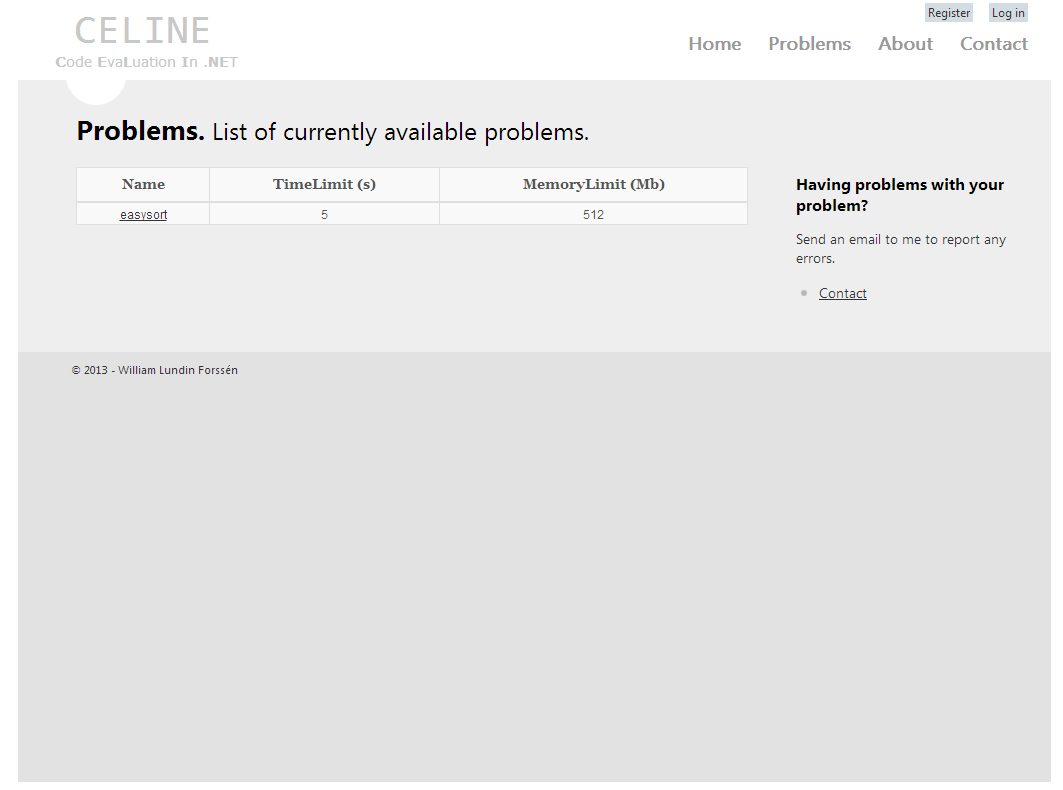
\includegraphics[width=0.48\textwidth]{chapters/media/celine_listproblems.png}
		\label{fig:celine_listproblems}
	}
	\subfigure[One problem called ``easysort''.]{
		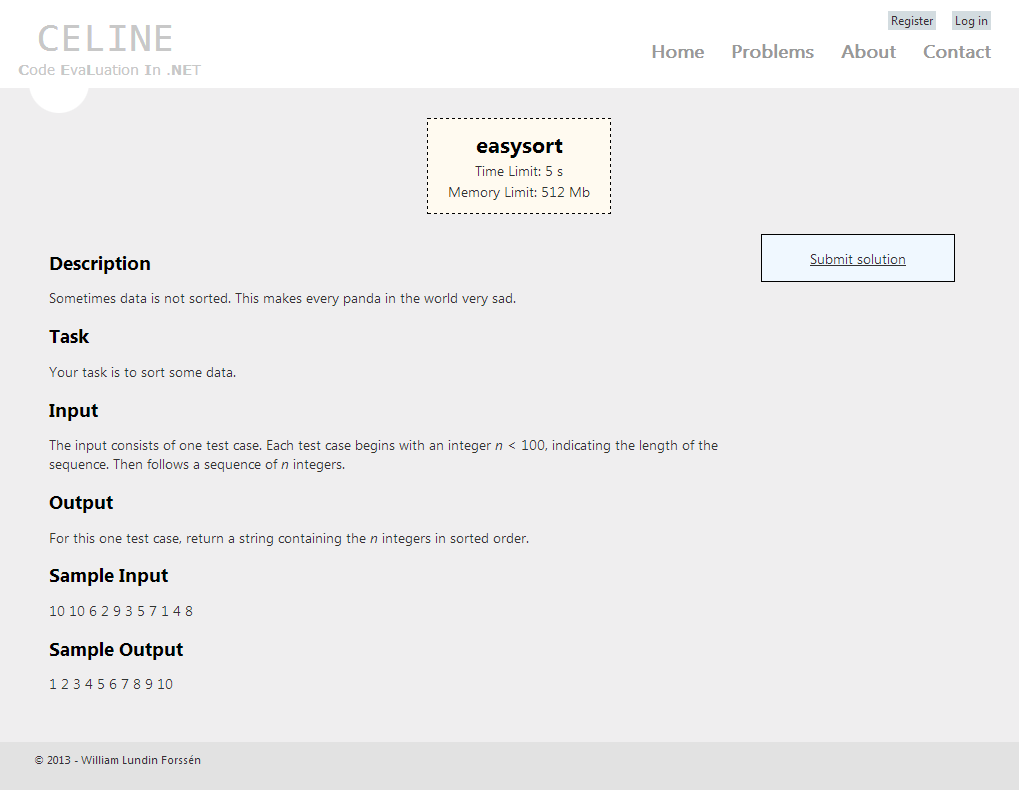
\includegraphics[width=0.48\textwidth]{chapters/media/celine_easysort.png}
		\label{fig:celine_easysort}
	}
}
\caption{Navigation in the Problems menu.}
\label{fig:celine_split_problemlist_easysort}
\end{figure}

Figure \ref{fig:celine_listproblems} shows what happens if you click on ``Problems'' in the menu. A list of currently available problems is displayed. The list contains details such as maximum run time and maximum memory usage. Clicking on one of the problems in this list will generate a page with more details of that particular problem, this is displayed in Figure \ref{fig:celine_easysort}. To the right of the details-text is a button for submitting a solution. Clicking it will generate a page containg a form for submitting code, illustrated in Figure \ref{fig:celine_submit}. Apart from the form itself on the left side, this page contains some useful information on the right side.

\begin{figure}[h]
\centering
\mbox{
	\subfigure[Code submission page.]{
		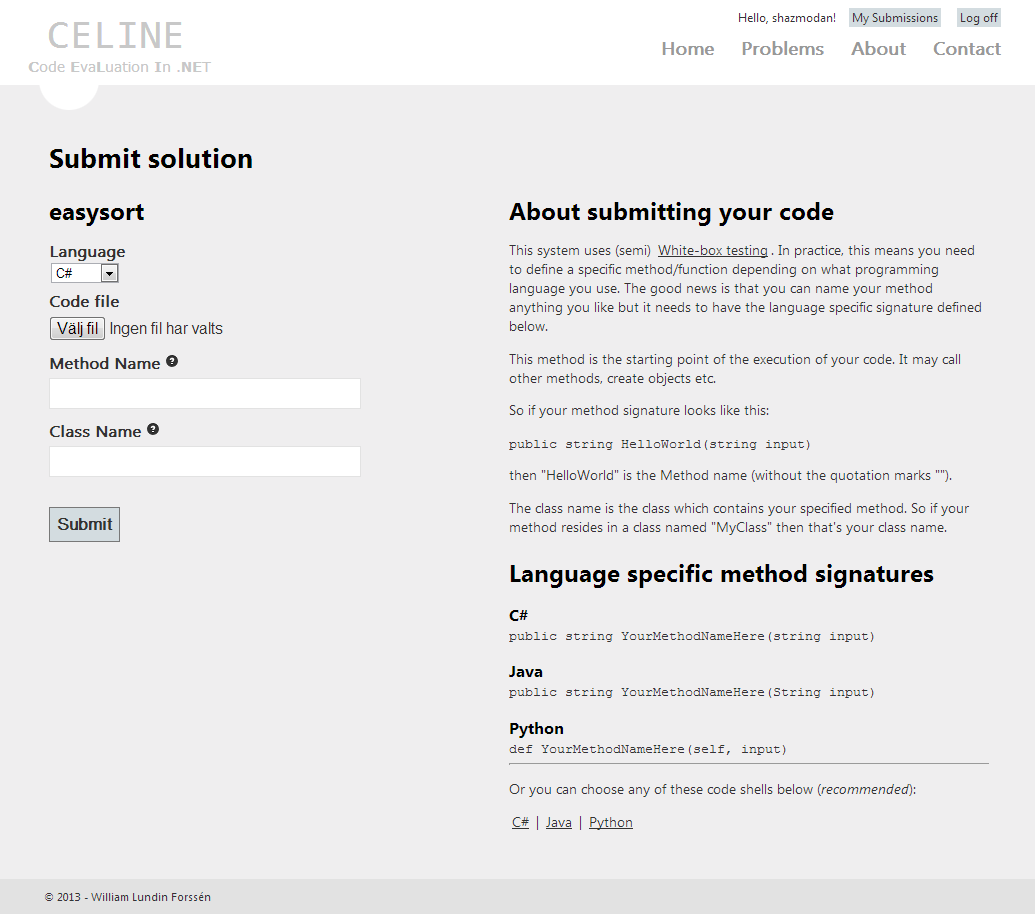
\includegraphics[width=0.48\textwidth]{chapters/media/celine_submit.png}
		\label{fig:celine_submit}
	}
	\subfigure[List of all submission made by the current user.]{
		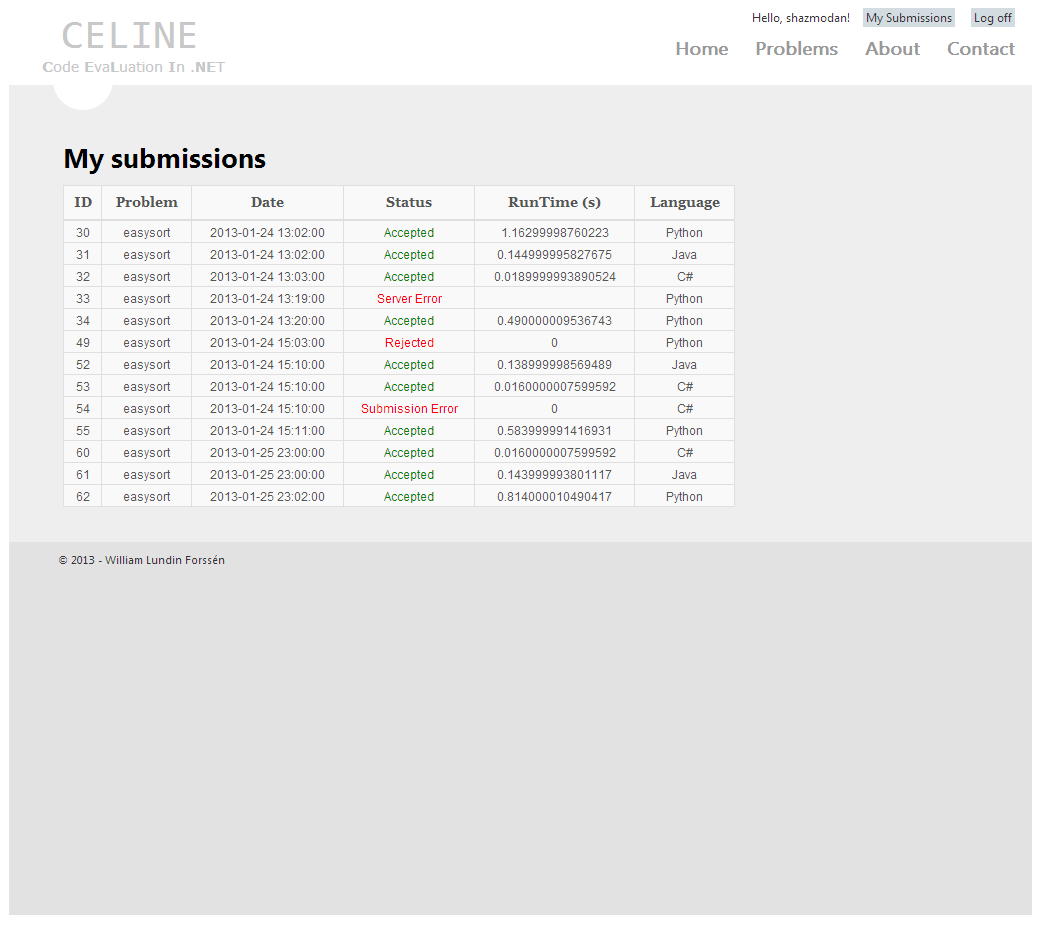
\includegraphics[width=0.48\textwidth]{chapters/media/celine_submissions.png}
		\label{fig:celine_submissions}
	}
}
\caption{Navigation when submitting code.}
\label{fig:celine_split_submit_submissions}
\end{figure}

Figure \ref{fig:celine_submissions} shows the page listing all of the current users submissions. The user is sent here after successfully submitting a solution (by filling out all the fields of the Submission page illustrated in Figure \ref{fig:celine_submit}) or by clicking on the button in the top right corner. This page contains information about each of the users submissions. Each line details what problem the user attempted to solve, a timestamp, total runtime, the programming language used and the returned status code. 



\subsection{The status codes} \label{subsec:status_codes}
The status code is a simple message indicating if the submission was successful or not. This system attempts to be more verbose on errors than other modern systems (described in section \ref{sec:todays_systems}) since it uses white-box testing which is more prone to submission related errors than black-box testing. These concepts are described more thoroughly in section ???. FIXME
\begin{itemize}
	\item Accepted - The code has compiled, run and gave the correct answer.
	\item Wrong Answer - The code has compiled and run but gave the wrong answer.
	\item Server Assembly Error - The CES failed to build an assembly from the codefile, thus making the code unable to run.
	\item Submission Error - Occurs if the code tries to reference a code library that isn't available/allowed. 
	\item Illegal Operation - Occurs if the CES detects a forbidden system call (i.e. accessing files, using the network etc...).
	\item Class or Function Error - Occurs if the class or method name doesn't correspond to the name provided by the user, thus resulting in the CES being unable to invoke the method.
	\item Time Limit Exceeded - The code ran longer than the limit for this particular problem.
	\item Rejected - This is a general error, it indicates that the CES has been unable to determine why the submission failed. 
	\item Server Error - This indicates that the CES instance has crashed.
\end{itemize}



\subsection{The code evaluation system}
When a user has submitted his or her code, it eventually reaches the CES. Figure \ref{fig:flowchart} describes the flow of the most common paths for a submission through the system.

\begin{figure}[h]
	\centering
	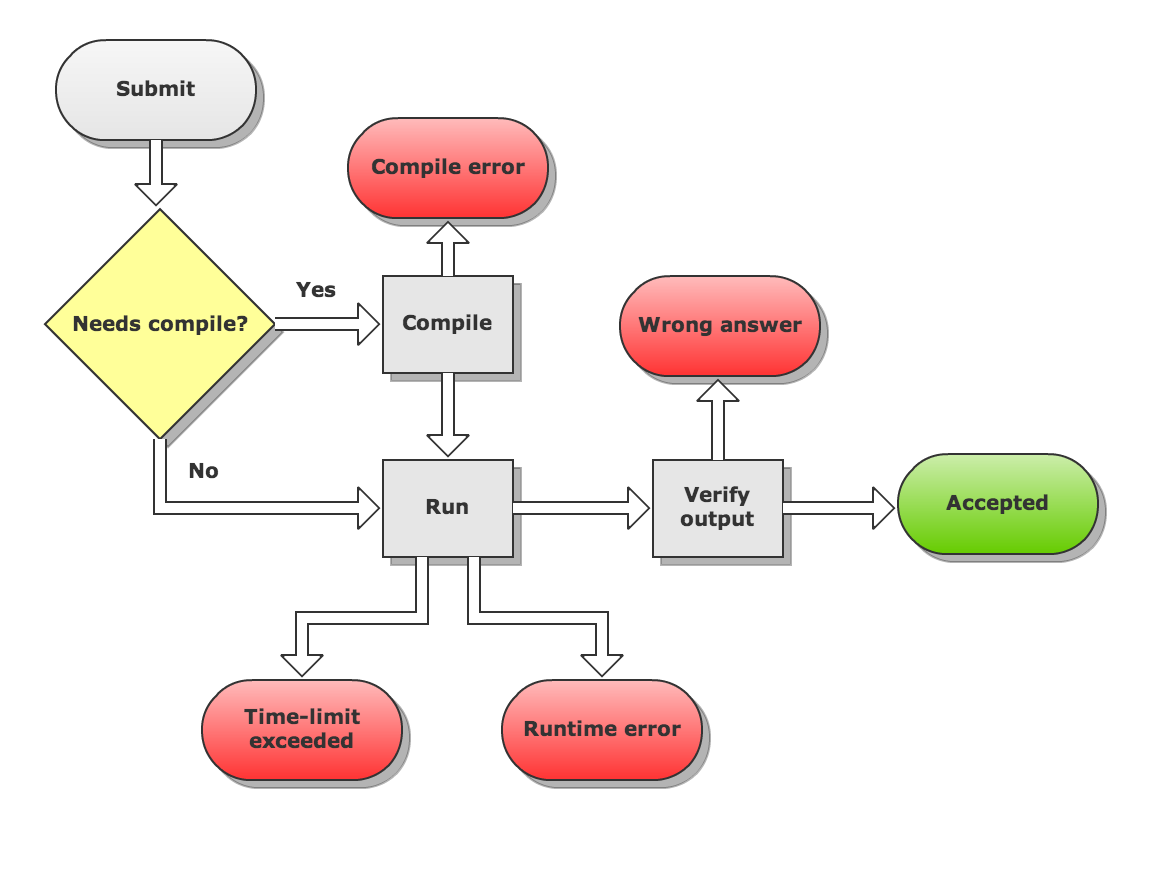
\includegraphics[width=0.8\linewidth]{chapters/media/flowchart.png}
	\caption{Common paths of problem flow in the CES.}
	\label{fig:flowchart}
\end{figure}

Depending on the programming language, a compiler is chosen. The code is then compiled into an assembly file and loaded into a seperate secure (sandboxed) Application Domain (AppDomain). The CES then invokes the user specified method with a string containing the test data. The CES waits for the code to complete or for the problem to timeout. It then compares the string returned by this method with another string containing what should be the correct output. If the strings match, the submission is regarded as being a success, otherwise it's regarded as a failure. The CES then returns the appropriate status code. 




